%%%% Class %%%%

% Class of the document: KOMA Script Article
%   Options: 12 points font, A4 paper, bibliography in ToC
\documentclass[a4paper,fontsize=10pt,bibliography=totoc]{scrartcl}

%%%% Preamble %%%%
% Packages inclusions
\usepackage[top=0.75in,bottom=1in,left=0.75in,right=0.75in]{geometry}								% Custom margins (comment out if not needed)
\usepackage[english]{babel}				% Language settings
\usepackage{lmodern}					% Use Latin Modern font
\usepackage[nointegrals]{wasysym}
\usepackage{microtype}					% Enhanced typesetting (better reading)
\usepackage{graphicx}					% Enhanced graphics processing
\usepackage{url}
\usepackage{breakurl}
\usepackage[table,hyperref,x11names,svgnames]{xcolor}				% Allows coloring tables
\usepackage[section]{placeins}			% Ensure float elems. inside their section
\usepackage{booktabs}					% Beautiful, "pro" tables
\usepackage{adjustbox}					% Boxing capabilities for images and text
\usepackage{multirow}					% Enables tabular cells spanning multiple rows
\usepackage{array}					% Enables custom table column defintions
\usepackage[toc,page]{appendix}			% Appendices title customisation
\usepackage{enumitem}					% Customized enumerations and itemizes
\usepackage[version=3]{mhchem}			% Allows inclusion of chemical formulas and eq.
\usepackage{amssymb}
\usepackage[ruled,vlined]{algorithm2e} % Algorithms and pseudocode
\usepackage{todonotes}					% Useful to put TODO side notes
\usepackage[noblocks]{authblk}			% Allows authors with affiliations
\usepackage{lastpage}					% Allows referencing the last page
\usepackage[style=british]{csquotes}    % Allows block quotations
\usepackage{titlesec}
\usepackage{nameref}	% Allows references by name ("Section 5" vs "Conclusions")
\usepackage{fancyhdr}					% Fancy headers and footers
\usepackage{multicol}
\usepackage{lipsum}
\usepackage[
	backend=biber,
	natbib=true,
	bibstyle=authoryear,
	citestyle=authoryear,
	sorting=nyt,
	block=space,
	hyperref=true,
	dashed=false
]{biblatex}
\usepackage{hyperref}
\hypersetup{
  unicode=true,
 	pdfpagemode={UseOutlines},
 	pdfstartview={FitV},
	bookmarks=true,
	bookmarksopen=true,
	bookmarksopenlevel=0,
	bookmarksnumbered=true,
	breaklinks=true, % to have links breaking among lines
	hypertexnames=true,
	plainpages=false,
	hidelinks=false,
	colorlinks=true,
	citecolor=Turquoise4,
	filecolor=black,
	linkcolor=DeepSkyBlue4,
	urlcolor=RoyalBlue3,
	anchorcolor=RoyalBlue3
}

% Command definitions
\makeatletter

% useful cross referencing commands
\newcommand{\fref}[1]{Figure~\ref{#1}}
\newcommand{\tref}[1]{Table~\ref{#1}}
\newcommand{\eref}[1]{Equation~\ref{#1}}
\newcommand{\cref}[1]{Chapter~\ref{#1}}
\newcommand{\sref}[1]{Section~\ref{#1}}
\newcommand{\aref}[1]{Appendix~\ref{#1}}
\newcommand{\alref}[1]{Algorithm~\ref{#1}}
\newcommand{\procref}[1]{Procedure~\ref{#1}}

\newcommand\frontmatter{%
	\cleardoublepage
	\pagenumbering{roman}}

\newcommand\mainmatter{%
	\cleardoublepage
	\pagenumbering{arabic}}

\newcommand\backmatter{%
	\cleardoublepage
}

\renewcommand\Authands{ and }

\newcommand{\norm}[1]{\lvert #1 \rvert}

\newcommand{\titlemake}[1]{%
		\begin{center}
%			\begingroup
				\Large\sffamily\bfseries{#1}
%			\endgroup
		\end{center}
}

\newcommand{\subtitlemake}[1]{%
	\begin{center}
		\begingroup
			\large\sffamily{#1}
		\endgroup
	\end{center}
}

\newcommand{\old}[1]{\textcolor{Red2}{#1}}

\makeatother

\newenvironment{checklist}{%
  \begin{list}{}{}% whatever you want the list to be
  \let\olditem\item
  \renewcommand\item{\olditem[$\Box$] }
  \newcommand\checkeditem{\olditem[$\CheckedBox$] }
}{%
  \end{list}
}

% Koma Script font modifications
\setkomafont{author}{\small}
\setkomafont{date}{\scshape}
\addtokomafont{section}{\large}
\addtokomafont{subsection}{\normalsize}
\addtokomafont{subsubsection}{\small}
\addtokomafont{caption}{\small}
\setlength{\abovecaptionskip}{2pt plus 0pt minus 2pt}
\setlist{nosep}
\renewcommand*{\bibfont}{\footnotesize}

% Formatting for paragraphs (indentation and space after par.)
\setlength{\parskip}{0.5\baselineskip}%
\setlength{\parindent}{1em}%

% Column separation
\setlength{\columnsep}{1.5em}

% Reduce space after sections
\titlespacing{\section}{0pt}{\parskip}{-0.5\parskip}
\titlespacing{\subsection}{0pt}{-0.25\parskip}{-0.6\parskip}
\titlespacing{\subsubsection}{0pt}{-0.5\parskip}{-0.75\parskip}

% Configuration of the blockquotes paragraphs
\SetBlockThreshold{0} % all blockquotes of 1 or more lines are treated as blocks

\addbibresource{references.bib}

%%%% Document %%%%

\begin{document}
% Page style set to fancy to get customized headers
\pagestyle{fancy}
\fancyhf{} % clear header and footer
\rhead{\footnotesize \today}
\lhead{\footnotesize David Martínez Rodríguez}
\chead{\footnotesize MSc Thesis Synopsis}
\rfoot{\footnotesize \thepage}

\titlemake{ % \titlemake[1] is a custom command -- look in the preface!
MSc Thesis Synopsis
}
%\subtitlemake{Extension of the CERO framework and policy assessment in Barcelona}

\begin{multicols}{2}

\section{Background}
\label{s:background}
Transport related airborne pollution is one of the main causes of respiratory diseases and associated increase in morbidity in densely populated areas~\parencite{vimercati2011_Trafficrelatedair,who2006_Airqualityguidelines}. The link from air pollution to both severe health problems and high traffic volumes is well known and thoroughly researched~\parencite{who2006_Airqualityguidelines}. However, an unsustainable transportation system not only causes health issues, but massive costs in terms of reduced productivity, freight delay, increased energy and fuel consumption or vehicle losses and damages, for example~\parencite{li-zeng2012_SocialCostTraffic}.

To address all these issues, \textit{policy} packages or simultaneous enforcing of different policies are needed, because of the complexity involved in effectively reducing transportation impacts~\parencite[ch. 3, p. 45]{garciasierra2014_Travelbehaviourenvironmental}. Regulation cannot, however, be designed without evaluating the caused impacts, at any level, in the short and long term -- too many resources and possible negative outcomes would be at stake. \textit{Policy assessment} from the systems thinking perspective is, therefore, a key issue to develop, due to the difficulty of dealing with entire systems, their internal dynamics and the emergent systemic behaviour patterns, such as feedback loops, rebound effects and hidden causalities. In this regard, the field of \textit{system dynamics} can help capture such structures and cause-effect chains \parencite{hjorth2006_Navigatingtowardssustainable}.

Finally, there is another perspective to be considered in the thesis. Policy development in the field of transportation has been mainly focused on two paths, according to \textcite{koehler2009_transitionsmodelsustainable}, to increase the sustainability of the system: (a) eco-efficiency increasing measures, by means of incentives for technological enhancements (e.g. better engines or fuel mixes) and more stringent pollution limits and (b) behavioural change management, i.e., measures aimed at modal shift -- encouraging people to shift from private cars to public transport, for example. Both approaches, albeit successful to some extent, have not delivered the expected results so far, due to the high inertia and stabilization mechanisms inherent to the current dominant regime for transportation: internal combustion engines cars-based mobility \parencite{geels2012_AutomobilityTransitionSocio}. However, a third way is possible, when it comes to policy design for sustainable mobility: \textit{transition management oriented policy} (TMOP).

In order to \colorbox{red}{TODO}, the approach of TMOP entails adopting a longer term thinking mindset (usually one or several generations), multi-level and multi-domain thinking, maintaining support for a large set of solutions and a focus in system \textit{innovation} alongside system improvements \parencite{rotmans2001_Moreevolutionthan}.

\section{Synopsis}
\label{s:synopsis}
\subsection*{Thesis title}
The proposed title for the thesis is: \textit{``Comparing eco-efficiency and transition management policies in the transport sector. A system dynamics approach.''}

\subsection*{Research question}
The research question that the thesis addresses is: \textit{``Can transition management oriented policies trigger better responses than eco-efficiency and behavioural oriented ones, when aiming for a more sustainable transport system?''}

\subsection*{Aim}
In order to answer the previous research question, an aim is set for the thesis: \textit{``To explore a method for system-wide evaluation of transition management policies targeting a more sustainable transport system''}.

\subsection*{Objectives}
The set of objectives designed to fulfil the aim of the thesis are:
\begin{enumerate}[label=(\alph*)]
	\item \textit{Identify} the important variables and system structures affecting transportation in urban areas, as well as the drivers and locking mechanisms of a potential transition towards a more sustainable transport system.
	\item \textit{Design} a conceptual model for the transportation system, including the previously identified social, environmental, economic and structural aspects.
	\item \textit{Quantify} the relations of the conceptual model to enable in-depth policy analysis.
	\item \textit{Validate} the model with regards to policy assessment and provide an example on how to use the model.
\end{enumerate}

\subsection*{Methods}
The chosen tool for the conceptual modelling step is the \textit{causal loop diagram} (CLD), probably followed by \textit{system dynamics} modelling in the quantification step, although this is still not clear\footnote{The final decision between implementing the quantification step through \textit{system dynamics} or \textit{agent-based modelling} will be based on literature research and a thorough justification of the strengths and weaknesses of each method.}. The models obtained using this technique are easy to understand by a majority of stakeholders, they quickly convey the interrelations of the main components of a (dynamic) system and, finally, they are useful to highlight the feedback structure of the modelled system~\parencite{ghosh2015_DynamicSystemsEveryone}. A more detailed plan of the methodology is depicted in the following enumeration:
%
\begin{enumerate}[label=(\alph*)]
	\item Perform a \textit{literature review} to retrieve the necessary data and knowledge about the diverse transportation system components.
	\item Design a \textit{conceptual CLD}, linking different components in the transport system. To achieve a highly comprehensive model, iteratively expand the system boundaries of the CLD by including other aspects that affect or are affected by the transport system, with the insights provided by the literature research.
	\item Using the collected data from the literature review, fit as many \textit{equations} as possible for the links in the model. The quantification is done in three steps:
	\begin{enumerate}[label=\roman*.]
		\item Identify and define the quantifiable links between \textit{core components} of the system.
		\item Quantify ``external'' links dealing with social issues, such as healthcare or accident costs, if enough data is available.
		\item Quantify the links from the core components of the system to the transition management assessment level.
	\end{enumerate}
	\item Validate the evaluation model through a \textit{case study} in either Barcelona or Stockholm\footnote{The choice of the city will depend on data availability and potential language barriers.}, assessing the city's mobility plans.
\end{enumerate}

\section{Thesis schedule}
\label{s:schedule}
The thesis preliminary schedule is shown in \tref{t:schedule}. The plan contemplates several phases, that will be broken down into the appropriate tasks within the \textit{Planning Report}, once a more clear roadmap is designed. A Gantt chart depicting the same schedule is shown in \fref{f:gantt-chart}. The phases of the thesis are designed to fit the main objectives of the study, as shown in \tref{t:schedule}.

\printbibliography
\end{multicols}

\begin{table}[h!]
\centering
\footnotesize
\caption{Thesis preliminary plan. Phases shown will be broken down into tasks in the planning report.}
\label{t:schedule}
\begin{tabular}{lllll}
\toprule
Task & Objective & Start date & End date & Duration (work)\textsuperscript{1} \\
\midrule
PH0 Thesis definition & -- & Jan 16 & Jan 20 & 5 d \\
PH1A Literature review & (a) & Jan 23 & Feb 3 & 10 d \\
PH1B Planning report writing & -- & Jan 30 & Feb 3 & 5 d \\
Planning report & -- & Feb 3 & Feb 3 & Milestone \\
PH2 Model development & (b), (c) & Feb 6 & Mar 31 & 40d \\
PH3 Model benchmark & (d) & Apr 3 & Apr 28 & 20 d \\
PH4 Report writing & -- & May 1 & May 26 & 20 d \\
Thesis report & -- & May 26 & May 26 & Milestone \\
PH5 Presentation preparation & -- & May 29 & Jun 6 & 7 d \\
Final presentation & -- & Jun 6 & Jun 6 & Milestone \\
\bottomrule
\end{tabular}
{\\ \scriptsize \parbox{0.7\linewidth}{\textsuperscript{1} Only \textit{work} days are included in the duration specification -- weekends are excluded from the calculation. Therefore, 20 days correspond to 4 full weeks (a month) worth of work.}}
\end{table}

\begin{figure}[h!]
\centering
\footnotesize
{\setlength{\fboxsep}{0pt}\fbox{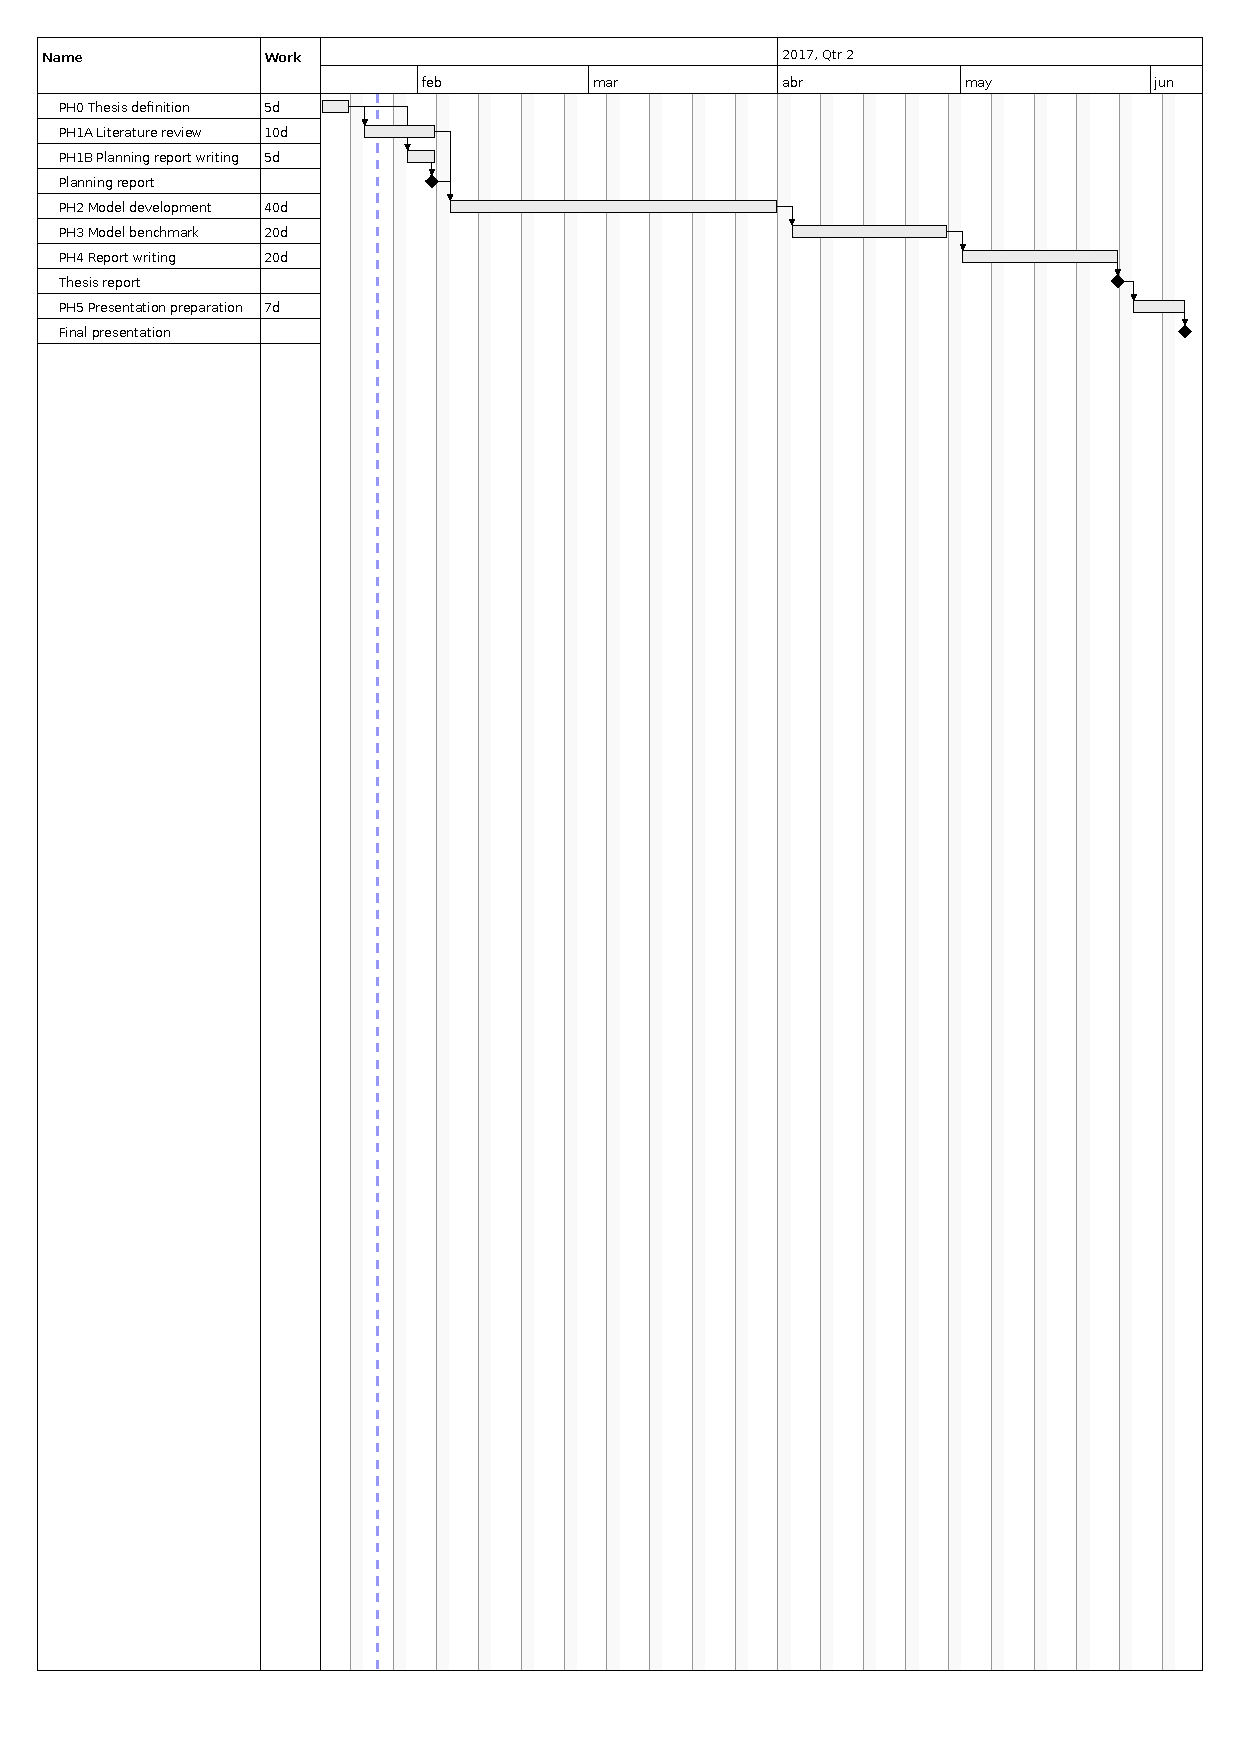
\includegraphics[width=\linewidth,clip,trim=0.64cm 23.9cm 0.7cm 0.7cm]{figures/thesis-gantt.pdf}}}
\caption{Thesis preliminary plan, as a Gantt chart. Milestones are marked with a $\blacklozenge$ symbol.}
\label{f:gantt-chart}
\end{figure}

\end{document}
